\section{Safety in Our Environment} \index{Safety}

\begin{multicols}{2}


\section*{Waste Disposal} \index{Waste disposal}


\subsection{Biodegradable Waste} \index{Biodegradable materials} % banana, bottle, etc in a hole

%\begin{center}
%\includegraphics[width=0.4\textwidth]{./img/.png}
%\end{center}

\begin{description*}
%\item[Subtopic:]{}
\item[Materials:]{Shovel/jembe, Banana peel, plastic bottle, rubber bands, paper}
%\item[Setup:]{}
\item[Procedure:]{Dig several small holes and place a different item in each, covering them with dirt. Check back on the items after several weeks, months, and after a year.}
%\item[Hazards:]{}
%\item[Questions:]{}
\item[Observations:]{The banana peel shrivels and degrades after a couple weeks, while the other items remain for many months or even years.}
\item[Theory:]{Banana peels are an example of organic waste. They are \emph{biodegradable}}, meaning that it breaks down in the environment. \emph{Non-biodegradable} waste does not break down, it just piles up.
\item[Applications:]{Do not throw plastic bottles out of the window on buses!!}
%\item[Notes:]{}
\end{description*}

\subsection{Planting Trees}

\begin{center}
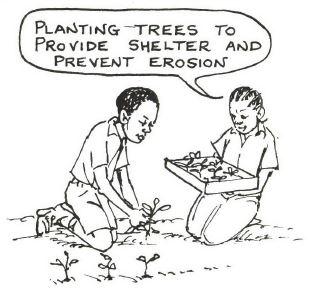
\includegraphics[width=0.4\textwidth]{./img/source/planting-trees.jpg}
\end{center}

\begin{description*}
%\item[Subtopic:]{}
%\item[Materials:]{}
%\item[Setup:]{}
\item[Procedure:]{Planting trees and protecting newly planted trees from animals is one way for community members to look out for the well-being of their environment and maintain and beautify their homes and schools.}
%\item[Hazards:]{}
%\item[Questions:]{}
%\item[Observations:]{}
\item[Theory:]{Trees consume excess carbon dioxide, which is a harmful greenhouse gas that eats away at our ozone layer. They produce the oxygen that we breath and help to maintain a balanced ecosystem for other organisms. }
\item[Applications:]{Many individuals cut down trees for firewood but fail to replace them with newly planted trees. Over time this can lead to erosion and degradation of the land.}
%\item[Notes:]{}
\end{description*}

\columnbreak

\subsection{Trash Journal} % Shika 242 

%\begin{center}
%\includegraphics[width=0.4\textwidth]{./img/.png}
%\end{center}

\begin{description*}
%\item[Subtopic:]{}
%\item[Materials:]{}
%\item[Setup:]{}
\item[Procedure:]{Have each student record in a journal all of the trash that they make every day for 2 weeks. If possible, collect the trash and weigh it every day.}
%\item[Hazards:]{}
\item[Observations:]{}
\item[Theory:]{Trash is a big problem in large towns and cities. Many manufactured goods come with a lot of waste material, which accumulates over time. Many waste items can be \emph{recycled}, or reused for different purposes.}
\item[Questions:]{What are some methods for eliminating waste? What effect does burning trash have on the environment?}
%\item[Applications:]{}
%\item[Notes:]{}
\end{description*}

\vfill

\subsection{Water Purity Surveys} \index{Water! purity}

\begin{center}
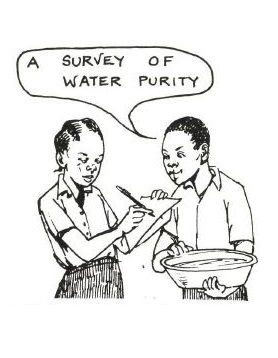
\includegraphics[width=0.4\textwidth]{./img/source/water-purity.jpg}
\end{center}

\begin{description*}
%\item[Subtopic:]{}
%\item[Materials:]{}
%\item[Setup:]{}
\item[Procedure:]{Keeping a record of water purity and health in a local community is a great way to raise awareness about environmental protection. Students can test for hardness of water, pH, or other impurities and harmful bacteria present in water samples.}
%\item[Hazards:]{}
\item[Questions:]{What are some other ways that you can get involved in protecting the environment?}
%\item[Observations:]{}
%\item[Theory:]{}
%\item[Applications:]{}
%\item[Notes:]{}
\end{description*}

%==================================================================================================%


\end{multicols}

\pagebreak